\documentclass{beamer}
\usetheme{Warsaw}
\useoutertheme{infolines}
\setbeamertemplate{headline}[default]
%\setbeamercovered{transparent}
%\setbeamertemplate{footline}[default]
%\setbeamertemplate{headline}[split]
\usepackage[T1]{fontenc}
\usepackage[utf8x]{inputenc}
\usepackage[english]{babel}
\usepackage{color}  
\usepackage{transparent}

%%%%%%%%%definition des variables%%%%%%%%%%%%%%%
%\usepackage[latin1]{inputenc}
%\usepackage[T1]{fontenc}
%\usepackage{textcomp}
%\usepackage{lmodern}
%\usepackage{listings} 


%%%%%%%%%%%%%%%%%%%%%%%%%%%%%
\def\sujet{}
\def\projet{LU decomposition on DAGuE} 
\def\etape{}
\def\gA{Omar \textsc{Zenati}, MsC Candidate}
\def\gB{Supervisors: M. Faverge, E. Agullo, G. Bosilca, P. Ramet}



%%%%%%%%%%%%%%%% Header %%%%%%%%%%%%%%%%
 \title[LU decomposition on DAGuE]{
        {\bfseries \projet\\} 
        {\bfseries \huge \sujet}
        {\small Friday Lunch Talk}
}


\titlegraphic{
  
\includegraphics[scale=0.5]{icl.png}
  \hfill
  
\includegraphics[scale=0.3]{inria.png}
  }
\date{May 25, 2012}

\author[Zenati]{
  {\normalsize \bfseries \sffamily} {\large \gA}\\
  \vspace{1cm}
  {\normalsize \bfseries \sffamily} {\large \gB}\\
}

\begin{document}
        
\begin{frame}
\maketitle
\end{frame}

\begin{frame}{Summary}
\tableofcontents
\end{frame}

\AtBeginSection[]{
  \begin{frame}{Summary}
  \tableofcontents[currentsection,subsectionstyle=shaded]
  \end{frame}
}

\AtBeginSubsection[]{
  \begin{frame}{Summary}
  \tableofcontents[currentsection,currentsubsection]
  \end{frame}
}

\section{LU Decomposition Algorithm}
\begin{frame}{Introduction}
\begin{itemize}
\item The need of LU decomposition algorithm
\item The evolution (linpack, lapack, scalapack, plasma, dplasma (mine))
\end{itemize}
\end{frame}

\begin{frame}{Introduction}
\framesubtitle{The algorithm}
\begin{itemize}
\item Display algorithm
\item Introduce the problem of accuracy
\end{itemize}
\end{frame}

\section{Static Pivoting and Iterative Refinement}

\begin{frame}{Static pivoting algorithm}
\begin{itemize}
\item Display algorithm
\item Show the advantages and the limits
\end{itemize}
\end{frame}


\begin{frame}{Static pivoting performance}
\end{frame}

\section{Partial Pivoting}

\begin{frame}{Partial pivoting algorithm}
\begin{itemize}
\item Display algorithm
\item Show the advantages and the limits
\end{itemize}
\end{frame}

\subsection{Panel Factorization}

\begin{frame}{Panel Factorization}
\framesubtitle{Comparative study}
\begin{itemize}
\item Natural Version
\item Implemented Version
\end{itemize}
\end{frame}

\begin{frame}{Panel Factorization}
\framesubtitle{Panel operations}
\begin{center}
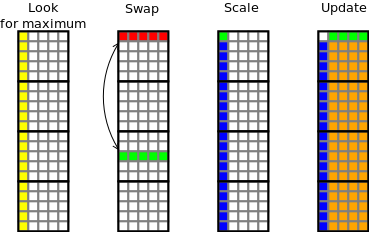
\includegraphics[scale=0.8]{panel_operation.png}
\end{center}
\end{frame}

\begin{frame}{Panel Factorization}
\framesubtitle{Look of maximum}
\begin{columns}
\begin{column}{.30\textwidth}
\begin{center}
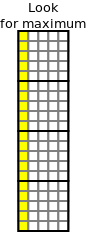
\includegraphics[scale=0.8]{panel_max.png}
\end{center}
\end{column}
\hfill
\begin{column}{.70\textwidth}
Each tile sends its maximum line to the main tile.
\begin{center}
\begin{exampleblock}{}
$\Longrightarrow$ Number of communications : $MT*NB$\\
$\Longrightarrow$ Number of tasks : $2*MT$
\end{exampleblock}{}
\end{center}
\end{column}
\end{columns}
\end{frame}

\begin{frame}{Panel Factorization}
\framesubtitle{Swap}
\begin{columns}
\begin{column}{.30\textwidth}
\begin{center}
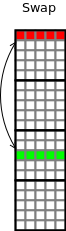
\includegraphics[scale=0.8]{panel_swap.png}
\end{center}
\end{column}
\hfill
\begin{column}{.70\textwidth}
Each tile need the new swap line.
\begin{center}
\begin{exampleblock}{}
$\Longrightarrow$ Number of communications : $MT*NB$\\
$\Longrightarrow$ Number of tasks : $MT$
\end{exampleblock}{}
\end{center}
\end{column}
\end{columns}
\end{frame}

\begin{frame}{Panel Factorization}
\framesubtitle{Scale and Update}
\begin{columns}
\begin{column}{.25\textwidth}
\begin{center}
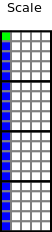
\includegraphics[scale=0.8]{panel_scale.png}
\end{center}
\end{column}
\hfill
\begin{column}{.25\textwidth}
\begin{center}
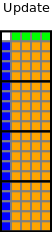
\includegraphics[scale=0.8]{panel_update.png}
\end{center}
\end{column}
\hfill
\begin{column}{.50\textwidth}
The two operations may be executed in the same task.
\begin{center}
\begin{exampleblock}{}
$\Longrightarrow$ the two operations are executed in the same task of the swap
\end{exampleblock}{}
\end{center}
\end{column}
\end{columns}
\end{frame}

\begin{frame}{Panel Factorization}
\framesubtitle{Comparative study}
\begin{itemize}
\item Natural Version
\begin{exampleblock}{}
\begin{itemize}
\item Total tasks : $2 * MT * NB * min(MB,NB)$
\item Total global communications : $2 * MT * min(MB,NB)$
\end{itemize}
\end{exampleblock}{}
\item Implemented Version
\end{itemize}
\end{frame}

\begin{frame}{Panel Factorization}
\framesubtitle{Implemented version}
\begin{columns}
\begin{column}{.70\textwidth}
Optimizations:
\begin{itemize}
\item Look for the maximum locally using thread parallelism
\item Share the local result by using a binary tree
\item Share the global result by using Bruck's algorithm
\item Use internal blocking
\end{itemize}
\end{column}
\hfill
\begin{column}{.30\textwidth}
\end{column}
\end{columns}
\end{frame}

\begin{frame}{Panel Factorization}
\framesubtitle{Implemented version}
\begin{columns}
\begin{column}{.70\textwidth}
Optimizations:
\begin{itemize}
\item Look for the maximum locally using thread parallelism
\transparent{0.4}
\item Share the local result by using a binary three
\item Share the global result by using Bruck's algorithm
\item Use internal blocking
\end{itemize}
\end{column}
\hfill
\begin{column}{.30\textwidth}
\begin{center}
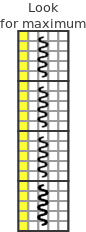
\includegraphics[scale=0.8]{panel_max_opt1.png}
\end{center}
\end{column}
\end{columns}
\pause
\begin{exampleblock}{}
$\Longrightarrow$ Number of tasks : $MT$
\end{exampleblock}{}
\end{frame}

\begin{frame}{Panel Factorization}
\framesubtitle{Implemented version}
\begin{columns}
\begin{column}{.70\textwidth}
Optimizations:
\begin{itemize}
{\transparent{0.4}
\item Look for the maximum locally using thread parallelism}
\item Share the local result by using a binary three
\transparent{0.4}
\item Share the global result by using Bruck's algorithm
\item Use internal blocking
\end{itemize}
\end{column}
\hfill
\begin{column}{.30\textwidth}
\begin{center}

\includegraphics[scale=0.6]{binary_reduction.png}
\end{center}
\end{column}
\end{columns}
\pause
\begin{exampleblock}{}
$\Longrightarrow$ Number of tasks : $MT$\\
$\Longrightarrow$ Number of local communications : $MT/P$
\end{exampleblock}{}
\end{frame}

\begin{frame}{Panel Factorization}
\framesubtitle{Implemented version}
\begin{columns}
\begin{column}{.50\textwidth}
Optimizations:
\begin{itemize}
{\transparent{0.4}
\item Look for the maximum locally using thread parallelism
\item Share the local result by using a binary three}
\item Share the global result by using Bruck's algorithm
\transparent{0.4}
\item Use internal blocking
\end{itemize}
\end{column}
\hfill
\begin{column}{.50\textwidth}
\begin{center}
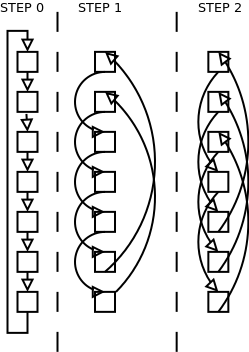
\includegraphics[scale=0.5]{bruck.png}
\end{center}
\end{column}
\end{columns}
\pause
\begin{exampleblock}{}
$\Longrightarrow$ Number of tasks : $log(P)$\\
$\Longrightarrow$ Number of global communications : $log(P)$
\end{exampleblock}{}
\end{frame}

\begin{frame}{Panel Factorization}
\framesubtitle{Implemented version}
\begin{columns}
\begin{column}{.50\textwidth}
Optimizations:
\begin{itemize}
{\transparent{0.4}
\item Look for the maximum locally using thread parallelism
\item Share the local result by using a binary three
\item Share the global result by using Bruck's algorithm}
\item Use internal blocking
\end{itemize}
\end{column}
\hfill
\begin{column}{.50\textwidth}
\begin{center}
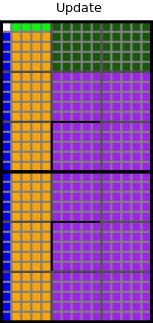
\includegraphics[scale=0.5]{panel_opt2.png}
\end{center}
\end{column}
\end{columns}
\end{frame}

\begin{frame}{Panel Factorization}
\framesubtitle{Comparative study}
\begin{itemize}
\item Natural Version
\begin{exampleblock}{}
\begin{itemize}
\item Total tasks : $2 * MT * NB * min(MB,NB)$
\item Total global communications : $2 * MT * min(MB,NB)$
\end{itemize}
\end{exampleblock}{}
\item Implemented Version
\begin{exampleblock}{}
\begin{itemize}
\item Total tasks : $(2 * MT + log(P)) * min(MB,NB)$
\item Total global communications : $log(P) * min(MB,NB)$
\end{itemize}
\end{exampleblock}{}
\end{itemize}
\end{frame}


\subsection{Update}

\begin{frame}{Update matrix}
\framesubtitle{Comparative study}
\begin{itemize}
\item Natural Version
\item Implemented Version
\end{itemize}
\end{frame}

\begin{frame}{Update matrix}
\framesubtitle{Natural version: Swap}
\begin{columns}
\begin{column}{.50\textwidth}
\begin{center}
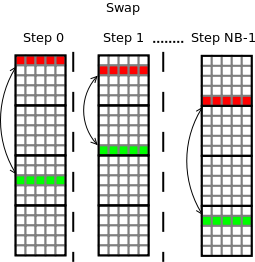
\includegraphics[scale=0.5]{update_swap.png}
\end{center}
\end{column}
\hfill
\begin{column}{.50\textwidth}
The main tile exchange swap lines with other concerned tile.
\pause
\begin{exampleblock}{}
$\Longrightarrow$ Number of tasks : $2*NB$\\
$\Longrightarrow$ Number of communications : $4*NB*NB$\\
$\Longrightarrow$ Difficult to implement in DAGuE
\end{exampleblock}{}
\end{column}
\end{columns}
\end{frame}

\begin{frame}{Update matrix}
\framesubtitle{Comparative study}
\begin{itemize}
\item Natural Version
\begin{exampleblock}{}
\begin{itemize}
\item Total tasks : $2 * NB * NT$\\
\item Total global communications : $4 * NB * NB * NT$
\end{itemize}
\end{exampleblock}{}

\item Implemented Version
\end{itemize}
\end{frame}

\begin{frame}{Update Matrix}
\framesubtitle{Implemented version}
\begin{columns}
\begin{column}{.50\textwidth}
Optimizations:
\begin{itemize}
\item Use of permutation instead of pivot index
\item Parallelize the swap from and the swap into the main tile
\end{itemize}
\end{column}
\hfill
\begin{column}{.50\textwidth}
\end{column}
\end{columns}
\end{frame}

\begin{frame}{Panel Factorization}
\framesubtitle{Implemented version}
\begin{columns}
\begin{column}{.70\textwidth}
Optimizations:
\begin{itemize}
\item Look for the maximum locally using thread parallelism
\transparent{0.4}
\item Share the local result by using a binary three
\item Share the global result by using Bruck's algorithm
\item Use internal blocking
\end{itemize}
\end{column}
\hfill
\begin{column}{.30\textwidth}
\begin{center}
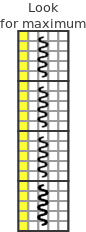
\includegraphics[scale=0.8]{panel_max_opt1.png}
\end{center}
\end{column}
\end{columns}
\pause
\begin{exampleblock}{}
$\Longrightarrow$ Number of tasks : $MT$
\end{exampleblock}{}
\end{frame}

\subsection{Performances}
\begin{frame}{Performances of partial pivoting}
\begin{itemize}
\item Shared memory
\item Problem scalability
\item Strong scalability
\end{itemize}
\end{frame}

\section*{Conclusion}
\begin{frame}{Conclusion and features}
\end{frame}

\end{document}
